\section{Locus of vertices of derived triangles}

A few triangles derived from billiard 3-periodics are shown in \cref{fig:05-derived-isosceles}. For their definitions see \cref{app:app-triangle} and \cite{mw}.

\begin{figure}
    \centering
    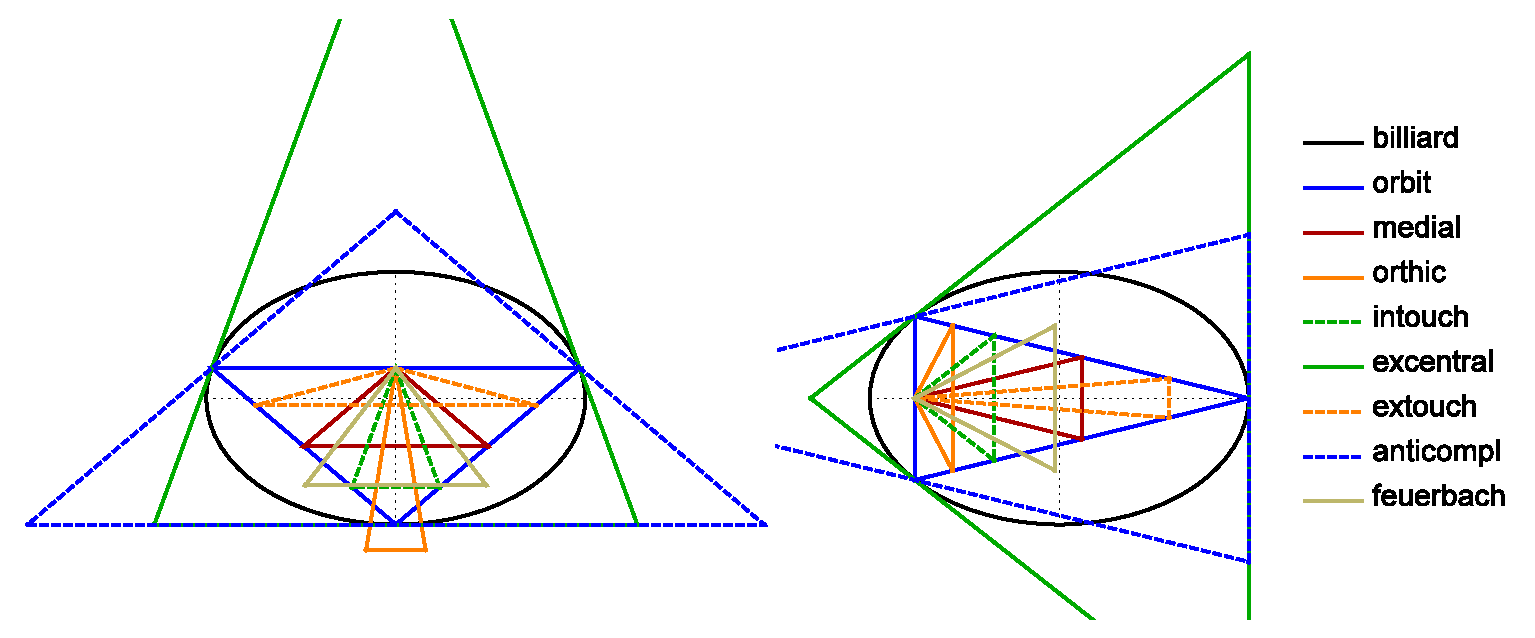
\includegraphics[width=\textwidth]{pics_05_100_confocal_derived}
    \caption{Triangles derived from an isosceles billiard 3-periodic (blue). These contain one vertex on the axis of symmetry. \href{https://youtu.be/xyroRTEVNDc}{Video}, \href{https://bit.ly/3fyylD0}{Live}}
    \label{fig:05-derived-isosceles}
\end{figure}

Mentioned in \cref{chap:01-intro} was an early experiment which showed that over billiard 3-periodics, the locus of the vertices of the intouch triangle (i.e., the intouchpoints) is a 2-lobed, self-intersect curve; see \cref{fig:01-intouch-locus}.

As shown in \cref{fig:05-locus-x11-x100}, the loci of vertices of some other triangles derived from billiard 3-periodics aren't ellipses. A noteworthy exception is the extouch triangle, mentioned above.

\begin{figure}
    \centering
    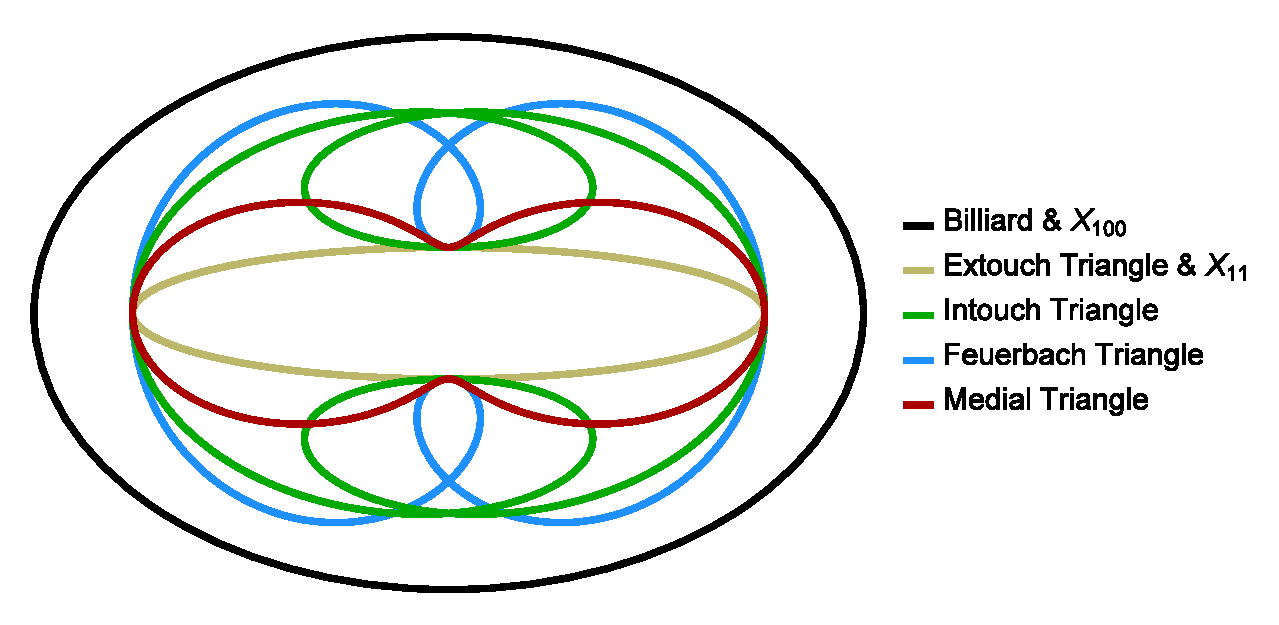
\includegraphics[width=\textwidth]{pics_05_070_non_elliptic}
    \caption{Non-elliptic loci of the vertices of triangles derived from billiard 3-periodics: the (i) intouch (green), (ii) Feuerbach (not to be confused with the Feuerbach {\em point}) (blue), (iii) medial (red), triangles. A noteworthy excpetion is the extouch triangle (light brown), whose vertices sweep the confocal caustic.
     \href{https://youtu.be/OGvCQbYqJyI}{Video}, \href{https://bit.ly/3orrSxQ}{Live}}
    \label{fig:05-locus-x11-x100}
\end{figure}
